\chapter{Towards high-performance network processing in virtualized environments\label{sec:HPCC}}

El artículo publicado se titula `` Towards high-performance network processing in virtualized environments '' y ha sido enviado al congreso HPCC, el cual está catalogado como \textbf{\href{http://103.1.187.206/core/?search=hpcc&by=all&source=CORE2014&sort=atitle&page=1}{CORE B}}. A continuación, se muestra la carta de aceptación, las revisiones y finalmente el artículo en sí.

\section{Email de aceptación}

\begin{verbatim}
 Fecha:	 6 de junio de 2015, 21:29:31 CEST
 De:	 HPCC 2015 <hpcc2015@easychair.org>
 Para:	 Víctor Moreno <victor.moreno@uam.es
 Asunto: HPCC 2015 notification for paper 51
\end{verbatim}
\begin{verbatim}
Dear Víctor,

Thank you for your contribution to IEEE HPCC 2015.

Congratulations! Your paper #51, titled as "Towards high-performance network
processing in virtualized environments", has been officially accepted as a
full paper for publication and presentation in IEEE HPCC 2015.

Please check reviewers' comments, and prepare your final version based on IEEE
conference proceeding format. The size of your final paper should be up to 6
pages complimentary, or 12 pages with the over length charge.

The completed reviews are attached below.

In order to publish your article, please prepare your final camera ready version
according to the requirements on IEEE HPCC website. 

We will send you the detailed instruction about your final submission in another
mail later.

Please prepare your trip (visa, air ticket, hotel) in advance. See you at
New York City.

Best,
PC Chairs of IEEE HPCC 2015
\end{verbatim}

\section{Revisiones}
\subsection{Revisor 1}
\begin{verbatim}
OVERALL EVALUATION: 0 (borderline paper)
REVIEWER'S CONFIDENCE: 4 (high)

----------- REVIEW -----------
This paper presents a study on some of the existing network processing techniques
in different configurations.  By comparing the package capturing capabilities and
performance, the authors claim that they provide the audience a series of guidelines
for network application deployment with low cost, high performance, space efficiency,
and low power consumption.

My major concern about the paper is its contribution. A large body of the paper is
devoted to presenting a preliminary investigation of several well known technologies
(PF_RING, Intel DPDK, HPCAP, etc.), omiting the detailed introduction to author's
own framework HPCAPvf.  The authors present their experimental results for various
configurations and techniques. However, I feel there is a lack of the experimental
details and methodology. To make their results more convincing, the authors should
include a methodology section dedicated to elaborate their experimental approach.
Too much space is taken to introduce the results, system structures and tradeoffs
for basic, well know concepts such as huge pages, package handling in virtualized
network, etc. Figure 4 and 5 take too much space.  The author should use more space
to introduce the details and techniques specific to this work.   Regarding the
presented results, why the authors use percentage of captured packages as a 
"perf!ormance" indicator of the compared techniques? I think this metric should be
used to indicate the accuracy, not the performance.

The paper is not well written. There are many typos and mistakes. Just to name a few:
In the sentence "traditional end-user network applications retrieves packets
individually by means of system calls, which in Linux systems involves at least two
context switches.", retrieves should be retrieve, involves should be involve.  This
sentence is long and reads awkward: "Those tests were made using the same hardware as
previously mentioned and using KVM for creating and managing the VMs, and accordingly
to the bare-metal scenario, the table depicts each capture engine’s performance for
the worst case scenario and in an average scenario.", and accordingly should be
according.  There are many other places that the author should do a proofreading.
\end{verbatim}

\subsection{Revisor 2}
\begin{verbatim}
OVERALL EVALUATION: 2 (accept)
REVIEWER'S CONFIDENCE: 2 (low)

----------- REVIEW -----------
This paper evaluates the performance of several well-known high-performance capture
engines on virtual machines. In addition, the paper presents an open-source version
of the HPCAP for virtual environments. The experimental results presented in this
paper are valuable for network operators that want to employ network virtual
functions.

The paper is well written and easy to understand even for a non-expert in this field.
The experimental results are based on a realistic benchmark and show insightful results.
\end{verbatim}

\section{Artículo}
Se adjunta el artículo completo en la siguiente página.

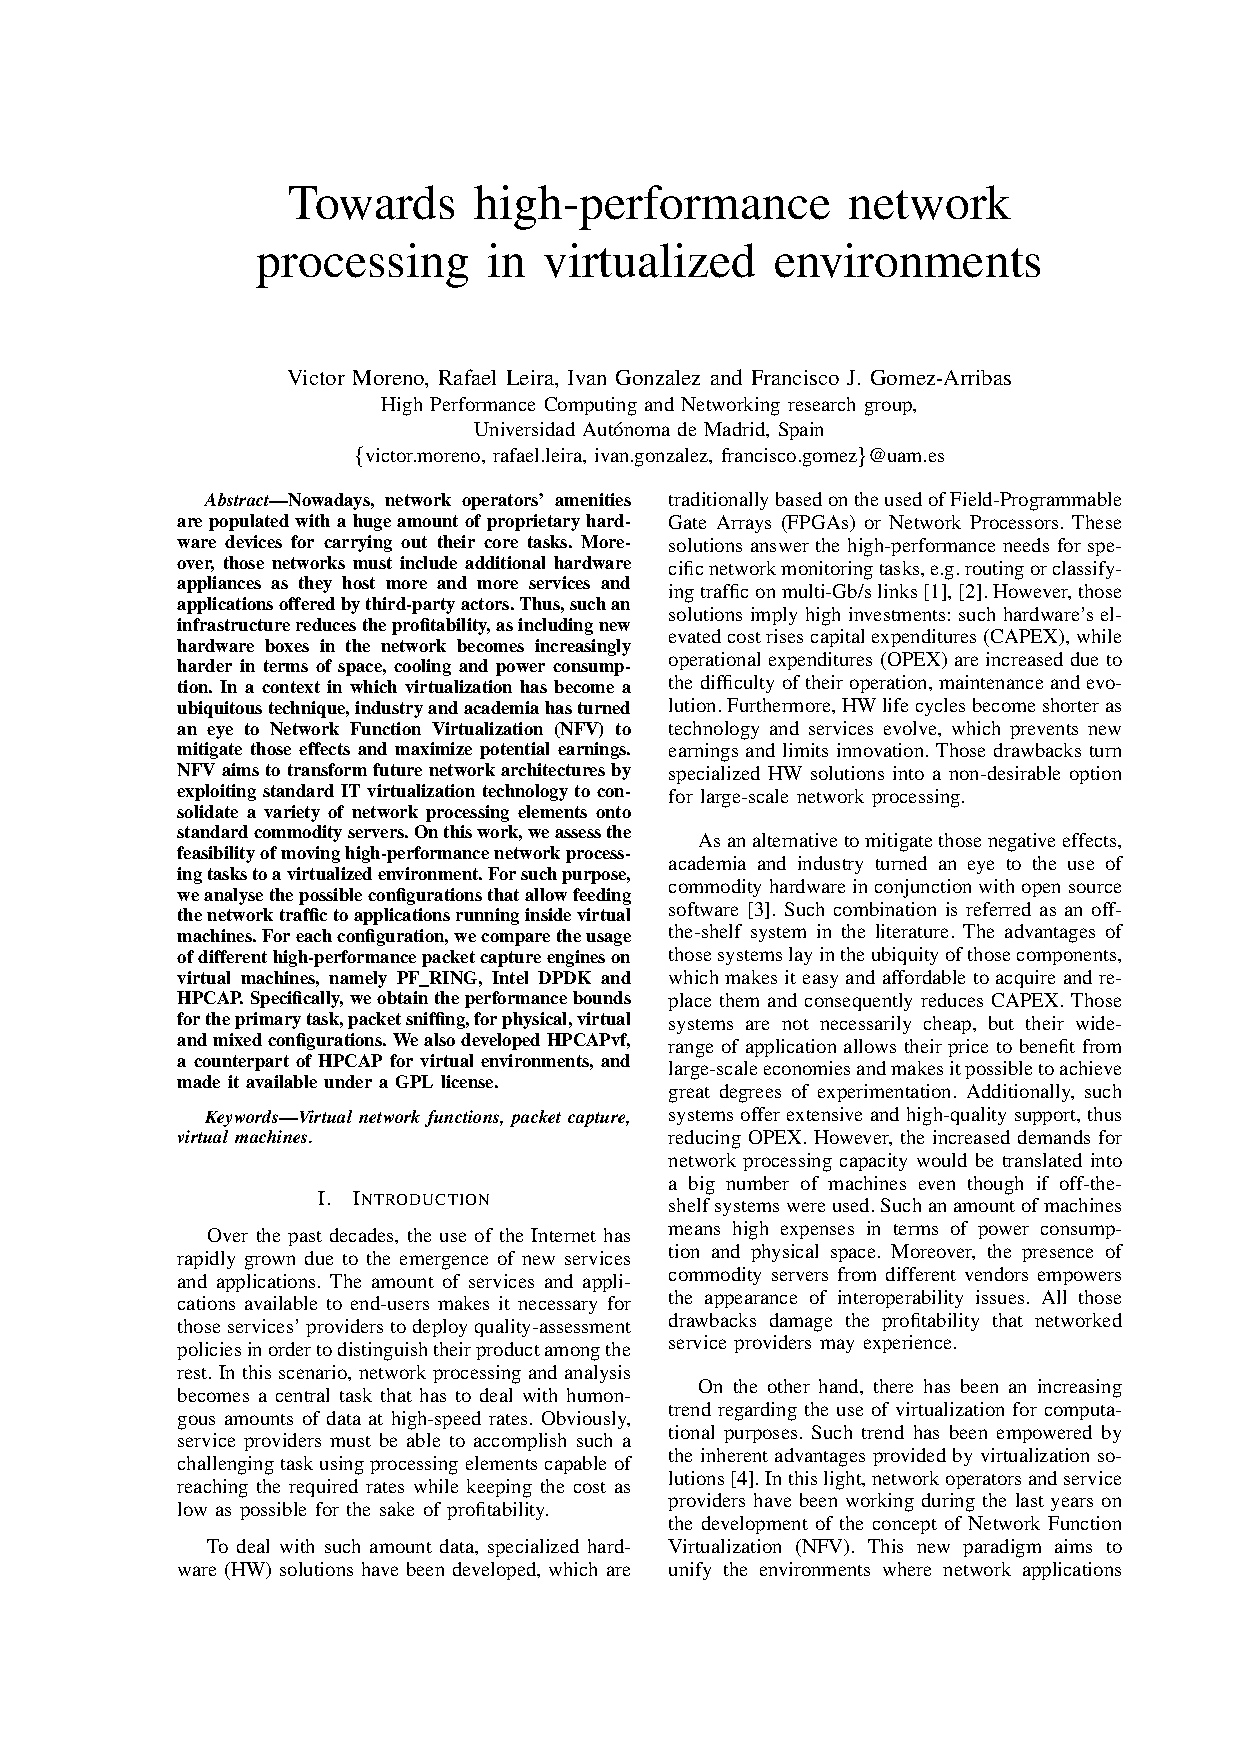
\includepdf[pages={1,2,3,4,5,6,7,8}]{graphics/virtualHPCC.pdf}